% Yunmo-Next-1B architecture. Build: tectonic figures/src/architecture.tex (then rendered to PNG).
\documentclass[tikz,border=4pt]{standalone}
\usepackage{amsmath}
\usepackage{newtxtext,newtxmath}
\usetikzlibrary{positioning,fit,arrows.meta,calc,backgrounds,decorations.pathreplacing}
\definecolor{gqa}{HTML}{D6E4F5}
\definecolor{kda}{HTML}{D8EFE3}
\definecolor{ffn}{HTML}{FBE3D2}
\definecolor{route}{HTML}{E6E1F5}
\definecolor{normc}{HTML}{F2F2EE}
\definecolor{edge}{HTML}{4A4A48}
\tikzset{
  box/.style={draw=edge, rounded corners=2pt, minimum height=6.2mm, minimum width=27mm, align=center,
              font=\footnotesize, line width=0.5pt},
  small/.style={box, minimum width=20mm, minimum height=5.4mm},
  arr/.style={-{Latex[length=1.6mm]}, line width=0.5pt, draw=edge},
  lbl/.style={font=\scriptsize, text=edge, align=left},
}
\begin{document}
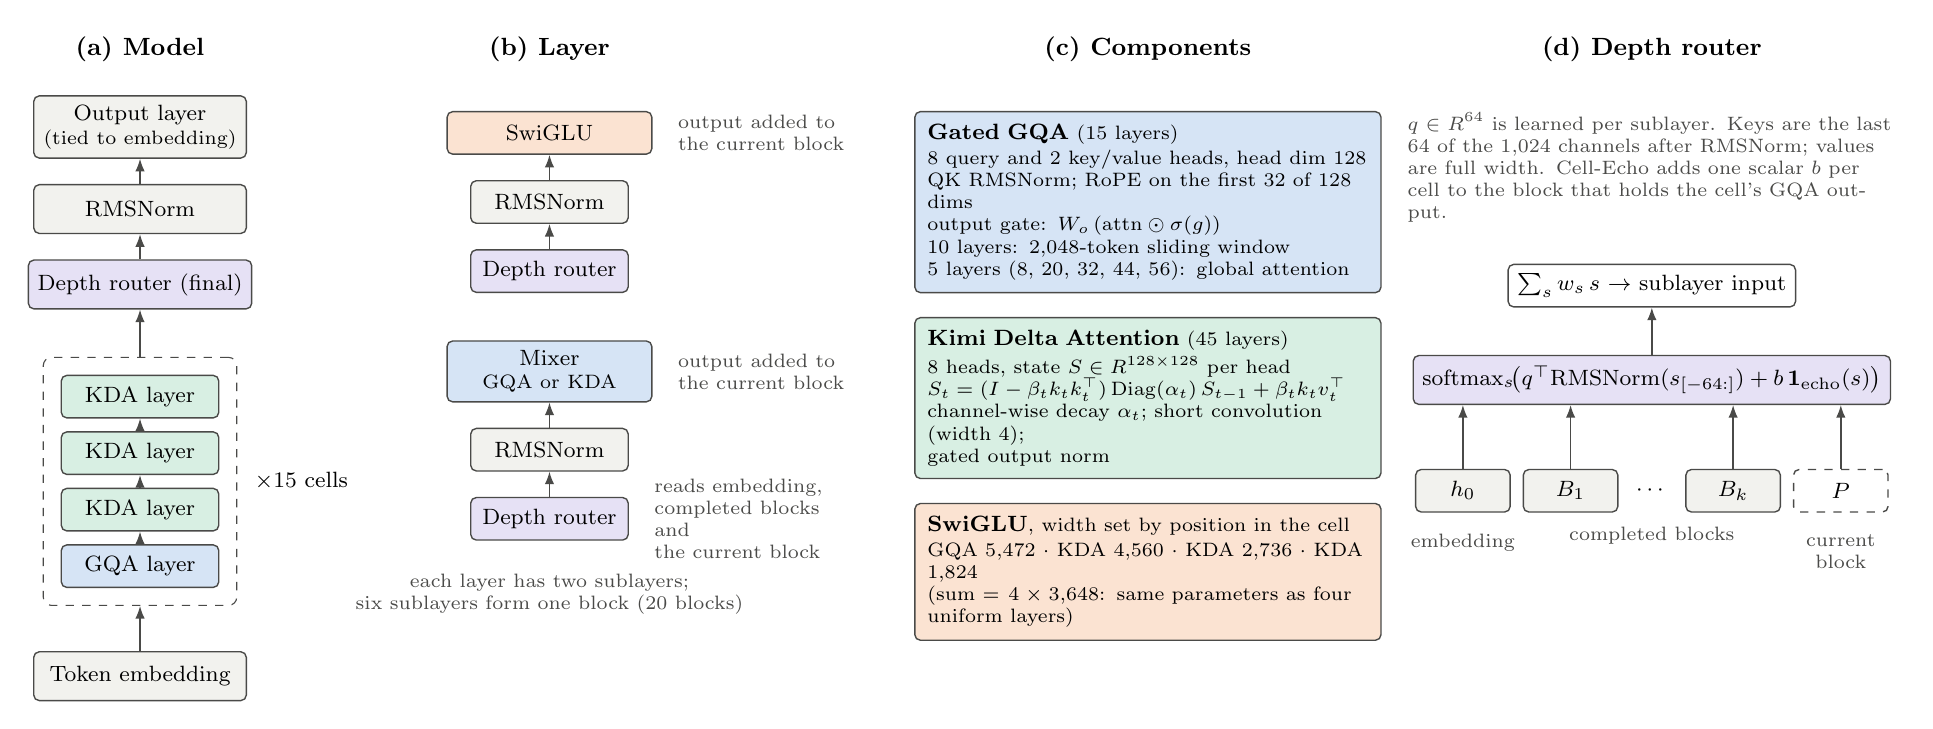
\begin{tikzpicture}[node distance=3.2mm]

% ---------------- (a) model stack ----------------
\node[box, fill=normc] (emb) {Token embedding};
\node[small, fill=gqa, above=8mm of emb] (l0) {GQA layer};
\node[small, fill=kda, above=1.6mm of l0] (l1) {KDA layer};
\node[small, fill=kda, above=1.6mm of l1] (l2) {KDA layer};
\node[small, fill=kda, above=1.6mm of l2] (l3) {KDA layer};
\node[draw=edge, rounded corners=3pt, dashed, fit=(l0)(l3), inner sep=2.2mm] (stack) {};
\node[font=\footnotesize, anchor=west] at ($(stack.east)+(1mm,0)$) {$\times 15$ cells};
\foreach \a/\b in {l0/l1,l1/l2,l2/l3} \draw[arr] (\a) -- (\b);
\node[box, fill=route, above=6mm of stack] (final) {Depth router (final)};
\node[box, fill=normc, above=of final] (fnorm) {RMSNorm};
\node[box, fill=normc, above=of fnorm] (head) {Output layer\\[-1pt]{\scriptsize (tied to embedding)}};
\draw[arr] (emb) -- (stack);
\draw[arr] (stack) -- (final);
\draw[arr] (final) -- (fnorm);
\draw[arr] (fnorm) -- (head);
\node[font=\small\bfseries, above=3mm of head] (ta) {(a) Model};

% ---------------- (b) one layer ----------------
\begin{scope}[xshift=52mm]
\node[font=\small\bfseries, anchor=center] (tb) at (0, 0 |- ta) {(b) Layer};
\node[small, fill=ffn, below=5mm of tb, minimum width=26mm] (mlp) {SwiGLU};
\node[small, fill=normc, below=of mlp] (n2) {RMSNorm};
\node[small, fill=route, below=of n2] (r2) {Depth router};
\node[small, fill=gqa, below=6mm of r2, minimum width=26mm] (mix) {Mixer\\[-1pt]{\scriptsize GQA or KDA}};
\node[small, fill=normc, below=of mix] (n1) {RMSNorm};
\node[small, fill=route, below=of n1] (r1) {Depth router};
\draw[arr] (r1) -- (n1); \draw[arr] (n1) -- (mix);
\draw[arr] (r2) -- (n2); \draw[arr] (n2) -- (mlp);
\node[lbl, right=2mm of mix] {output added to\\the current block};
\node[lbl, right=2mm of mlp] {output added to\\the current block};
\node[lbl, right=2mm of r1, text width=24mm] {reads embedding,\\completed blocks and\\the current block};
\node[lbl, below=3mm of r1, align=center] {each layer has two sublayers;\\six sublayers form one block (20 blocks)};
\end{scope}

% ---------------- (c) components ----------------
\begin{scope}[xshift=128mm, comp/.style={draw=edge, rounded corners=2pt, line width=0.5pt, text width=56mm,
      align=left, inner sep=1.6mm, font=\scriptsize}]
\node[font=\small\bfseries] (tc) at (0, 0 |- ta) {(c) Components};
\node[comp, fill=gqa, below=5mm of tc] (g) {\textbf{\footnotesize Gated GQA} (15 layers)\\[1pt]
   8 query and 2 key/value heads, head dim 128\\
   QK RMSNorm; RoPE on the first 32 of 128 dims\\
   output gate: $W_o\,(\mathrm{attn}\odot\sigma(g))$\\
   10 layers: 2{,}048-token sliding window\\
   5 layers (8, 20, 32, 44, 56): global attention};
\node[comp, fill=kda, below=3mm of g] (k) {\textbf{\footnotesize Kimi Delta Attention} (45 layers)\\[1pt]
   8 heads, state $S\in\mathbb{R}^{128\times128}$ per head\\
   $S_t=(I-\beta_t k_t k_t^{\top})\,\mathrm{Diag}(\alpha_t)\,S_{t-1}+\beta_t k_t v_t^{\top}$\\
   channel-wise decay $\alpha_t$; short convolution (width 4);\\ gated output norm};
\node[comp, fill=ffn, below=3mm of k] (f) {\textbf{\footnotesize SwiGLU}, width set by position in the cell\\[1pt]
   GQA 5{,}472 $\cdot$ KDA 4{,}560 $\cdot$ KDA 2{,}736 $\cdot$ KDA 1{,}824\\
   (sum $=4\times3{,}648$: same parameters as four uniform layers)};
\end{scope}

% ---------------- (d) depth router ----------------
\begin{scope}[xshift=192mm]
\node[font=\small\bfseries] (td) at (0, 0 |- ta) {(d) Depth router};
\node[lbl, below=4mm of td, text width=62mm, align=left] (note) {$q\in\mathbb{R}^{64}$ is learned per sublayer. Keys are the last 64 of the 1{,}024 channels after RMSNorm; values are full width. Cell-Echo adds one scalar $b$ per cell to the block that holds the cell's GQA output.};
\node[small, fill=white, below=4mm of note, minimum width=30mm] (out) {$\sum_s w_s\, s$ $\rightarrow$ sublayer input};
\node[box, fill=route, minimum width=52mm, below=6mm of out] (sm) {$\mathrm{softmax}_s\!\big(q^{\top}\mathrm{RMSNorm}(s_{[-64:]}) + b\,\mathbf{1}_{\mathrm{echo}}(s)\big)$};
\draw[arr] (sm) -- (out);
\node[font=\footnotesize, below=9mm of sm] (sd) {$\cdots$};
\node[small, fill=normc, minimum width=12mm, left=1mm of sd] (s1) {$B_1$};
\node[small, fill=normc, minimum width=12mm, left=1.5mm of s1] (s0) {$h_0$};
\node[small, fill=normc, minimum width=12mm, right=1mm of sd] (sk) {$B_{k}$};
\node[small, fill=white, dashed, minimum width=12mm, right=1.5mm of sk] (sp) {$P$};
\node[lbl, below=1.5mm of s0, align=center] {embedding};
\node[lbl, below=1.5mm of sd, align=center] {completed blocks};
\node[lbl, below=1.5mm of sp, align=center] {current\\block};
\foreach \s in {s0,s1,sk,sp} \draw[arr] (\s.north) -- (\s.north |- sm.south);
\end{scope}

\end{tikzpicture}
\end{document}
